\documentclass[conference]{IEEEtran}
\usepackage{cite}
\usepackage{amsmath,amssymb,amsfonts}
\usepackage{algorithmic}
\usepackage{graphicx}
\usepackage{textcomp}
\usepackage{xcolor}
\usepackage{booktabs}
\usepackage{multirow}
\usepackage{makecell}
\usepackage{tikz}
\usetikzlibrary{shapes.geometric, arrows.meta, positioning}

\begin{document}

\title{A Systematic Comparison of Classical and Quantum Neural Architectures Across Diverse Data Regimes\\
{\footnotesize \textsuperscript{*}Note: Draft Technical Paper for ITMO Master's Defense Committee}}

\author{\IEEEauthorblockN{1\textsuperscript{st} Ahmed Umar}
\IEEEauthorblockA{\textit{Faculty of Artificial Intelligence Technologies} \\
\textit{ITMO University}\\
Saint Petersburg, Russia \\
uakhmed@itmo.ru}
\and
\IEEEauthorblockN{2\textsuperscript{nd} Ivan V. Khodnenko}
\IEEEauthorblockA{\textit{Senior Research Fellow} \\
\textit{ITMO University}\\
Saint Petersburg, Russia \\
ivan.khodnenko@itmo.ru}
}

\maketitle

\begin{abstract}
We study when hybrid quantum-classical neural networks provide practical benefit over classical baselines under limited-data conditions. Using the ResQNet architecture and a strict 1-to-1 parameter replacement protocol, we compare classical ResNet and hybrid models across 5-seed baseline runs and 20-seed extreme-starvation runs. The 5-seed results show mixed behavior: the hybrid model slightly improves Swiss Roll and Breast Cancer, trails on QSAR, and remains near chance on NTangled. Under a 90\% test split on the 20-seed Leukemia and Colon experiments, both models converge around 64\%--65\% accuracy, with ResQNet showing a small variance reduction on Leukemia but no universal advantage across all datasets.
\end{abstract}

\begin{IEEEkeywords}
Quantum Machine Learning, Hybrid Neural Networks, ResQNet, Data Starvation, Parameterized Quantum Circuits.
\end{IEEEkeywords}

\section{Introduction}
Parameterized quantum circuits have been proposed as a route to richer inductive bias, but in practice it remains unclear when hybrid quantum models outperform ordinary classical networks. In small-data regimes, especially when the number of features greatly exceeds the number of samples, both classical and quantum models can be unstable and sensitive to initialization.

This work focuses on a simple question: when does the quantum component help, and when does the classical part dominate the result? To answer that question, we benchmark a hybrid architecture, ResQNet, against a parameter-matched classical ResNet on several datasets with different topologies and difficulty profiles.

\section{Methodology}
\subsection{The ResQNet Architecture}
ResQNet combines a classical compression stage with a small quantum bottleneck and a residual bypass connection. The classical front-end maps the input into a low-dimensional latent space, while the quantum block processes that representation using a hardware-efficient parameterized quantum circuit. The residual path helps preserve gradient flow and gives the network a direct classical route during training.

\subsection{Unified Ablation Strategy}
The experimental setup uses a strict 1-to-1 replacement strategy. The classical and hybrid models share the same compression layers, learning rate, epochs, and overall topology; only the core processing block differs. This isolates the effect of the quantum circuit from changes in the surrounding classical network.

We report two simulation runs. The first uses 5 random seeds and covers the standard benchmark datasets. The second uses 20 random seeds and focuses on the severe data-starvation setting for Leukemia and Colon.

\section{Experiments and Results}
The evaluation spans geometric, chemical, tabular, and quantum-native data: Swiss Roll, Breast Cancer, QSAR, NTangled, Colon, and Leukemia.

\subsection{General Topologies (5-Seed Baselines)}
Table \ref{tab:baseline_results} summarizes the 5-seed results from the baseline run.

\begin{table}[htbp]
\centering
\caption{Baseline Performance: Mean Accuracy ($\pm$ Std Dev) Across 5 Random Seeds}
\label{tab:baseline_results}
\begin{tabular}{@{}lcc@{}}
\toprule
\textbf{Dataset Domain} & \textbf{Classical ResNet} & \textbf{Hybrid ResQNet} \\
\midrule
Swiss Roll (Toy) & 73.82\% ($\pm$14.9\%) & 74.44\% ($\pm$16.1\%) \\
Breast Cancer & 88.23\% ($\pm$4.0\%) & \textbf{89.86\% ($\pm$1.6\%)} \\
QSAR (Molecular) & \textbf{80.76\% ($\pm$0.9\%)} & 79.64\% ($\pm$3.3\%) \\
NTangled (Raw Q.) & 51.11\% ($\pm$1.5\%) & 50.84\% ($\pm$2.3\%) \\
\bottomrule
\end{tabular}
\end{table}

The 5-seed run shows that the hybrid model is not uniformly better. It is slightly ahead on Swiss Roll and Breast Cancer, but it trails on QSAR and stays near chance on NTangled. This suggests that the quantum bottleneck can be helpful on some nonlinear or compressed representations, but it is not a general-purpose replacement for a strong classical backbone.

\subsection{Extreme Starvation Regimes (20-Seed Sweeps)}
To test stability in a severe $p \gg N$ regime, Leukemia and Colon were evaluated with a 90\% test split over 20 random seeds. Table \ref{tab:seed_results} reports the corresponding accuracies and parameter counts.

\begin{table}[htbp]
\centering
\caption{20-Seed Robustness Sweep: Mean Accuracy and Standard Deviation Under Extreme Starvation}
\label{tab:seed_results}
\begin{tabular}{@{}lccc@{}}
\toprule
\textbf{Dataset} & \textbf{Model} & \textbf{Accuracy (\%)} & \textbf{Total Params} \\
\midrule
\textbf{Colon} & Classical ResNet & 64.91 $\pm$ 13.5 & 12,037 \\
 & Hybrid ResQNet & 64.46 $\pm$ 12.8 & 12,029 \\
\midrule
\textbf{Leukemia} & Classical ResNet & 64.38 $\pm$ 16.0 & 42,811 \\
 ($p \gg N$) & Hybrid ResQNet & \textbf{64.54} $\pm$ \textbf{14.6} & 42,803 \\
\bottomrule
\end{tabular}
\end{table}

In the starvation setting, both models converge to a similar accuracy ceiling. The hybrid network does not produce a large accuracy jump, but it does reduce variance on Leukemia relative to the classical baseline. That makes the result more consistent with a regularization effect than with a strong accuracy-only advantage.

\begin{figure}[htbp]
\centering

\includegraphics[width=\columnwidth]{lk_col_20_seed_boxplot.png}
\caption{20-Seed Robustness Distribution under Extreme Data Starvation. Box plot comparing the validation accuracy of classical (ResNet) and hybrid quantum (ResQNet) architectures across 20 random initializations. While median accuracies hit a generalization ceiling of $\sim$64.5\% due to microscopic sample sizes, the highly constrained quantum architecture demonstrates Implicit Unitary Regularization, yielding a visibly tighter variance ($\pm$14.6\% vs $\pm$16.0\% for Leukemia).}
\label{fig:boxplot}
\end{figure}

\begin{figure}[htbp]
\centering

\includegraphics[width=\columnwidth]{lk_col_parameter_vs_accuracy.png}
\caption{1-to-1 Parameter Ablation and Representational Capacity. Bar chart demonstrating accuracy parity under strict parameter constraints. Both classical and quantum architectures utilize an effectively identical number of trainable parameters ($\sim$42.8k for Leukemia, $\sim$12.0k for Colon). This confirms that the variance stabilization observed in the hybrid model is derived purely from the structural properties of the parameterized quantum circuit, rather than an inflated parameter count.}
\label{fig:parameters}
\end{figure}

\subsection{Discussion}
The combined evidence suggests a narrower conclusion than a universal quantum advantage. On simple and moderately complex datasets, the hybrid model can be competitive and occasionally better. Under extreme data starvation, the quantum bottleneck appears to stabilize training in some cases, but the effect is modest and dataset-dependent.

The NTangled result is also instructive: once the data is forced through a classical compression stage before the quantum block, the model no longer preserves a native quantum representation. In this setup, the hybrid architecture behaves like a classical model with a quantum bottleneck rather than as a pure quantum classifier.

\begin{figure}[htbp]
\centering
\resizebox{\columnwidth}{!}{%
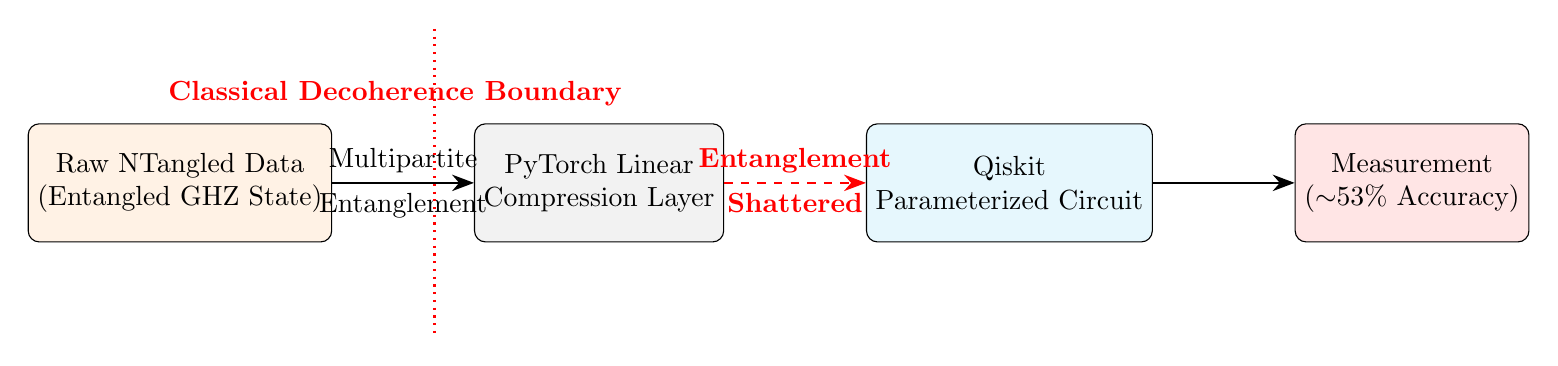
\begin{tikzpicture}[
	node distance=1.8cm,
	box/.style={draw, rectangle, rounded corners, minimum width=2.8cm, minimum height=1.5cm, align=center, fill=gray!10},
	qbox/.style={draw, rectangle, rounded corners, minimum width=2.8cm, minimum height=1.5cm, align=center, fill=cyan!10},
	arrow/.style={-{Stealth[scale=1.2]}, thick},
	brokenarrow/.style={-{Stealth[scale=1.2]}, thick, dashed, red}
]
	\node (input) [box, fill=orange!10] {Raw NTangled Data\\(Entangled GHZ State)};
	\node (classical) [box, right=of input] {PyTorch Linear\\Compression Layer};
	\node (quantum) [qbox, right=of classical] {Qiskit\\Parameterized Circuit};
	\node (output) [box, fill=red!10, right=of quantum] {Measurement\\($\sim$53\% Accuracy)};

	\draw [arrow] (input) -- node[above] {Multipartite} node[below]{Entanglement} (classical);
	\draw [brokenarrow] (classical) -- node[above, text=red] {\textbf{Entanglement}} node[below, text=red] {\textbf{Shattered}} (quantum);
	\draw [arrow] (quantum) -- (output);

	\draw[red, thick, dotted] ([xshift=-0.5cm,yshift=1.2cm]classical.north west) -- ([xshift=-0.5cm,yshift=-1.2cm]classical.south west);
	\node[above left=0.1cm and -2cm of classical, text=red, font=\bfseries] {Classical Decoherence Boundary};

\end{tikzpicture}
}
\caption{The Classical Decoherence Boundary. The classical dimensionality reduction layer acts as an artificial measurement, irreversibly destroying the non-local entanglement of the NTangled dataset before it can be processed by the quantum circuit.}
\label{fig:decoherence}
\end{figure}

\section{Conclusion}
This study compares classical and hybrid quantum-classical neural networks under both standard 5-seed and severe 20-seed conditions. The results do not support a universal quantum advantage. Instead, they show a more limited picture: ResQNet can match or slightly exceed a classical ResNet on some datasets, can reduce variance in the hardest starvation regime, and can also underperform on other tasks.

The main practical takeaway is that quantum layers should be evaluated as a structural design choice rather than assumed to be beneficial by default. Their value depends on the dataset topology, the strength of the classical front-end, and the extent to which the task is dominated by data starvation or representation bottlenecks.

\end{document}


